\chapter{Introduction}
\label{cha:intro}
\epigraph{The best weapon of a dictatorship is secrecy, but the best weapon of a democracy should be the weapon of openness.} 
{\textit{Niels Bohr}} 

\section{Problem Statement}

A democracy can be described as a system where all eligible voters have equal rights to express their opinion(s) on different matters. 
One of the most important example of expressing the opinion is holding elections to elect the leader of country. During the 
elections, all eligible voters express their opinion on a paper, also known as ballot,	 in a manner, depending on the voting method, 
which reflects their true opinion. For example, if the voting method is \textit{ranked voting (preferential voting)}, then the voters rank the 
candidates according to their preference, and if the method is \textit{first past the post}, then each voter selects one candidate by marking
against the candidate name in the ballot. Later, once the ballot cast finishes, a candidate is elected as a winner from  the participating
candidates by combing the choices of all the voters. 
The paper ballot method works great, except it is very time consuming, expensive, error prone, 
and not very inclusive for disabled voters such as visually impaired.
In order to solve the various problems posed by paper ballot, many countries are adopting electronic voting as an alternative. 
Electronic voting is 
getting popular in many countries, and the reason for its popularity is cost-effective, faster result, high voter turn out, 
and accessible for disabled voters.  
Undeniably, electronic voting has helped, for example, Australia to ease the logistic challenges of elections because of its massive land size and sparsely 
population and save millions of dollars.  In addition, it has helped India, the second most populous country with 900 million eligible voter, to declare 
2019 election with 67 percent voter turn out (roughly 600 million) in 2 days, and  Estonia, a labour shortage country, has saved 
thousands of man hours, 11,000 working days, by using electronic voting \citep{Estonia}.

   
  Despite all these benefits, electronic voting is an arduous effort because a minuscule possibility of 
  going anything wrong in software or hardware could lead to a disaster,   possibly 
  inverting the results \citep{TSwiss},
  \citep{10.1007/978-3-319-22270-7_3}, \citep{ARANHA2019335},
  \citep{Feldman:2007:SAD:1323111.1323113}.  The nature of (electronic) data and ease of 
  its manipulability/misinterpretation causes electronic voting many problems, which are not present in paper ballot elections, that 
  makes it perfectly susceptible to delivering wrong and unverifiable result \citep{Wolchok:2010:SAI:1866307.1866309}.
  For instance,  if a software program used in electronic voting 
  for reading the ballots has byte order bug, or even if it depends on some other software which has byte order bug (the data is suppose to read 
  from left to right, but software is reading right to left), then the interpretation of 
  ballot would completely be different from what the voter had in mind.
  More often than not, these software programs are configured incorrectly \citep{1301313} and run at the top of (untrusted) operating 
  system and hardware. Usually, operating systems have millions of lines code (Linux has 15 millions lines) which exposes
  a large attack surface and could be exploit, possibly by current government or foreign countries, for illegal gain.
  The worst, these software and hardware  are commercial in 
  confidence and treated as a black-box, and, most often, their source code or design is not open 
  for public scrutiny \citep{AEC:2013:LMM}. In addition, these software programs 
  take a list of ballots and produce the result without producing any evidence about the correctness of result.  As a consequence,
  from casting the ballot electronically and declaring winner based on cast (electronic) ballot, the whole process lacks basic assumptions
  of democracy such as transparency, genuineness, and verifiability. 
  
  In order to make the electronic voting process genuine and trustworthy, electronic voting 
  research community has recognized some must have properties of electronic voting protocol
  \citep{5958051}, 
   \citep{Benaloh:1994:RSE:195058.195407},  \citep{Delaune:2010:VPT}, \citep{Bernhard:2017:PES}:
  

 \begin{itemize}
 
  \item Correctness:
 	The produced results are correct, and convincing to all leaving no  ground for suspicion. 

 \item Coercion-resistance: A voter can not cooperate with a coercer to prove anything about her choices.
 
 \item Eligibility: Only eligible voter can cast the ballot.
 	
 \item Privacy:
    All the votes must be secret, and voter should not be able to convince anyone the 
    value of her vote.
 
 \item End-to-end Verifiability:
 Any independent third party should be able to verify the final outcome of election based on cast 
 ballots.  It can be further divided into three sub-categories:
 
 \begin{itemize}
  \item Cast-as-intended: Every voter can verify that their ballot was cast as
  intended.
  \item Collected-as-cast: Every voter can verify that their ballot was collected as
  cast.
  \item Tallied-as-cast: Everyone can verify final result on the basis of the
  collected ballots.
\end{itemize}
\end{itemize}
	

In this thesis, we focus on privacy, correctness, coercion-resistance, and tallied-as-cast, the third part of end-to-end verifiability, property 
of an election. Furthermore, we assume that the first two properties of end-to-end verifiability, \textit{cast-as-intended} and 
\textit{collected-as-cast}, hold for an election. \textit{Cast-as-intended} is a verification method that is is used to audit the 
front end voting software, 
also known as voting client software, to make sure that it is not modifying the options of voters. In a nutshell, 
the cast-as-intended is assurance to a voter that front-end software is transparent and her vote 
is recorded according to her intent.  \textit{Cast-as-intended} is itself an active area of research in its own right; 
however, it is not the focus of this thesis. Similarly, \textit{Collect-as-cast} is a notion related to the voters to make 
sure that the ballots appearing on the bulletin board are indeed the ballots that cast during the election. A consequence 
of \textit{collected-as-cast} notion is that any attempt to change or delete the ballots from the bulletin board would 
be detected. This notion is indeed a crucial one and works as a bridge between cast-as-intended and tallied-as-cast 
notion. However, it is related to voters' behaviour; hence, the reason for assumption.  Moreover, assuming these two 
notions, cast-as-intended and collected-as-cast, helped us in isolating the irrelevant details and 
paved a way to focus on more complex problem of counting, i.e. tallied-as-cast. 


\section{Research Motivation and Contribution}
Given the potential advantages of electronic voting,  we need to address
the correctness, privacy, and verifiability concerns for its widespread adoption. 
This thesis sets out to address these concerns of electronic voting. 
The questions we asked ourself was:
 \begin{enumerate} 
  \item Can we implement a vote counting protocol with the  
    "guaranteed" correctness
    of the implementation and practical enough
    to count the real life election involving millions of ballots (Correctness)?
  \item Can we produce the result by counting encrypted ballot without revealing 
  its content, and at the same time, 
  assuring everyone that the result produced is only based on "valid" ballots, 
  and "invalid" ones have been discarded  (Privacy and Coercion-resistance)?
 \item Can we decouple the verifiability from implementation, i.e. 
    generating enough evidence so that any independent auditor can 
    ascertain the outcome of election without trusting the implementation 
    of software used to conduct the election (Verifiability)?
  \end{enumerate}


In order to answer these questions, at first we need two things: (i) a voting protocol and 
(ii) a tool to implement the voting protocol and prove the correctness properties of the implementation. 
Our choice of voting protocol is the   Schulze method \citep{Schulze:2011:NMC} and 
the tool is Coq \citep{Bertot:2004:ITP} theorem prover  for implementing and proving 
the correctness of  Schulze method.
Even though Schulze method is not used in any democratic election to public office,
it has many interesting properties and, 
 at the same time, it is non-trivial.  
While no preferential voting scheme can guarantee all desirable properties that one would
like to impose due to Arrow’s theorem \citep{Arrow:1950:DCS}, the Schulze method offers a good compromise, 
with a number of important properties already  established  in  Schulze’s  original  paper. 
Amongst the various  properties, Schulze method satisfies the \textit{resolvability criterion}, 
i.e. elects a single winner under the assumption that number of voters are much larger than
 number of candidates (and in case of tie, when there are more than one winner, a random vote can be 
selected to declare winner.  However, our formalization 
has not taken the randomness into account, so it can produce more than one winner). 
Coq is a theorem prover (proof assistant) based on \textit{Calculus of Inductive Construction} 
\citep{Coquand:1988:CC:47724.47725} \citep{coquand1988inductively}. 
The \textit{Calculus of Inductive Construction} allows the "proof" terms and 
"computation" terms to live in the same universe (level), which leads to a highly expressive type 
system. Moreover, during the proof development, 
it provides a step by step feedback to the user and possibility to automate the proofs by 
writing the custom tactics using the Ltac \citep{10.5555/1765236.1765246}. In addition, 
Coq proofs can be extracted into the  Haskell, OCaml, and Scheme.
 
Now that we have a voting protocol (Schulze method) and  a tool (Coq theorem prover), 
we demonstrate that it is possible to achieve correctness, privacy, coercion-resistance, and (tallied-as-cast) verifiability in 
electronic voting. We achieve the following:
\begin{itemize}
 \item \textit{Correctness} by formally specifying the Schulze method  and prove its correctness properties
  inside the Coq theorem prover. 
 Coq has a well developed extraction facility that 
 we use to extract proofs into OCaml programs, and using these extracted OCaml programs, we 
 have counted the ballots from election to produce the result. 
 \item \textit{Privacy and Coercion-resistance} by encryption. We use homomorphic encryption to compute the 
  finally tally without decrypting any individual ballot. 
\item \textit{Verifiability} by tabulating the relevant data of election (we call it scrutiny-sheet/certificate).
   Achieving verifiability in a plain-text ballot counting is fairly straight forward.  
   To achieve verifiability in encrypted ballot counting, 
   we augment the scrutiny sheet with zero-knowledge-proof for the each claim we make during the 
   counting which can  later be checked by any auditor.  
\end{itemize}



\textit{Formally Verified Checker:} Third party independent election audit based on scrutiny sheet data is a crucial step towards 
establishing the trust in the system.   However, auditing scrutiny sheet of a election involving encrypted ballots
is not straight forward in comparison to  a election with plain-text ballots. 
In general, auditing scrutiny sheet of a election involving 
plain-text ballot simply requires the knowledge of basic arithmetic, e.g. addition, subtraction and multiplication, 
and virtually anyone can audit the election based on the data produced in the scrutiny sheet by
using a calculator or by writing a simple program in her preferred language. 
However, encrypted ballot election scrutiny sheet involves various
cryptographic concepts (homomorphic encryption, zero knowledge proof, commitment scheme, etc.) 
which are accessible to a very few voters, mainly cryptographers,  so auditing it 
requires deep understanding of cryptographic principals. To ease this situation, we have developed a formally verified 
certificate checker as a proof of concept for automating the auditing an election conducted on encrypted ballots. 
Having said that,  our certificate generated by encrypted ballots is very complex, and formalizing all the cryptographic 
primitives involved would be fairly time consuming, so we have developed a proof of concept 
formally verified certificate checker for International Association of Cryptographic Research 2018 election
scrutiny sheet, relatively simple than ours. 

\textit{Properties of Schulze Method:} We have proved couple of the properties, Condercet winner, and Reversal symmetry, 
of the Schulze method inside Coq theorem prover (ongoing work).
 

\section{Cryptographic Blackbox}
Since the beginning of this project, our primary goal was 
to achieve privacy (using encryption) and verifiability (using zero knowledge proof) in electronic voting 
using the cryptographic primitives (but not the verification of primitives itself). 
To achieve this goal, we have 
taken the axiomatic approach and assumed the existence of cryptographic primitives 
inside Coq. Moreover, we assume the axioms about their correctness behaviour, e.g. 
decryption is left inverse of encryption. These primitives, in general, provide functionality 
of generating a random permutation, encrypting a plain-text, decrypting a cipher-text, 
producing commitment of a value, constructing a zero-knowledge-proof, 
and verifying a zero-knowledge-proof. Later, in extracted OCaml code from Coq code, these functions are instantiated 
with Unicrypt \citep{LocherH14} function. 
\footnote{Formalizing the whole cryptographic stack used in our 
project would be very time consuming (probably a PhD itself), but it would be worth trying. 
Although, we have formalized the (El-Gamal) encryption, and decryption inside Coq, but we still 
are very far from achieving the goal of fully verified cryptographic stack.  We leave the formalisation 
of cryptographic primitives for future work (work in progress).}



\section{Publication}
 The chapters, or some part of it,  of this thesis are based on the following papers:
	\begin{enumerate}
	\item Pattinson, D. and Tiwari, M., 2017. Schulze Voting as Evidence carrying computation. In Proc. 
	ITP 2017, vol. 10499 of Lecture Notes in Computer Science, 410–426. Springer. 
	\item Lyria Bennett Moses, Rajeev Goré, Ron Levy, Dirk Pattinson, Mukesh Tiwari.
	No More Excuses: Automated Synthesis of Practical and Verifiable Vote-Counting Programs for Complex 
	Voting 	Schemes. E-VOTE-ID 2017: 66-83
	\item Milad K. Ghale, Rajeev Goré, Dirk Pattinson, Mukesh Tiwari.
	Modular Formalisation and Verification of STV Algorithms. E-Vote-ID 2018: 51-66
	\item Thomas Haines, Dirk Pattinson, and Mukesh Tiwari. 2019. 
	  Verifiable Homomorphic Tallying for the Schulze Vote Counting Scheme. 
	  11th International Conference Verified Software: Theories, Tools, and Experiments. 
      VSTTE 2019 (to appear)	  
	\item Thomas Haines, Rajeev Goré, and Mukesh Tiwari. 2019. Verified Verifiers for Verifying Elections. 
	 In Proceedings of the 2019 ACM SIGSAC Conference on Computer and Communications Security (CCS '19).
	\end{enumerate}
 \noindent
 Part of chapter \ref{cha:background} is based on \textit{No More Excuses: Automated Synthesis of Practical 
 and Verifiable Vote-Counting Programs for Complex Voting  Schemes},
 chapter \ref{cha:schulze_method} is based on \textit{Schulze Voting as Evidence Carrying Computation},
 chapter \ref{cha:homormorphic_schulze} is based on \textit{Verifiable Homomorphic Tallying for the 
 Schulze Vote Counting Scheme}, and part of chapter
 \ref{cha:software_independence} is based on \textit{Verified Verifiers for Verifying Elections}.




\section{Related Work}
 There is extensive work that 
 addresses the different issues related of electronic voting protocols  in symbolic model, 
 but there are very few, to the best of my knowledge, 
 that have used theorem provers to implement the voting protocol (counting algorithm)
 and verify its correctness properties. 
 \citep{10.1007/978-3-540-31987-0_14}, and  \citep{Delaune2010} have used pi-calculus, a formalism for describing concurrent systems,
 to model and analyse various properties, such as fairness, eligibility, vote-privacy, receipt-freeness and 
 coercion-resistant,  
 of the protocol FOO developed by \citep{10.1007/3-540-57220-1_66}.  \citep{Backes:2008:AVR:1380848.1381255}
 presented a general technique to model  remote electronic 
 voting protocol and automatically verifying  its security properties using pi-calculus. 
 \citep{5992139} have used pi-calculus to analyse the ballot secrecy of \citep{Helios:2016:HVS}.
 \citep{10.1007/978-3-642-28641-4_7} have used pi-calculus to ascertain the properties of 
 Norwegian electronic voting protocol.
 \citep{10.1007/978-3-319-68687-5_7} have used Tamarin  to prove receipt-freeness 
 and vote-privacy of Selene voting protocol \citep{Selene}.  Most of these work differs from ours
 in the sense that their primary focus is verification of security protocol in  
 Dolev-Yao model or  complexity-theoretic model, whereas our work is 
 more focused on verified implementation and  verifiability  aspect of vote counting.

 The closest to our work is \citep{Cochran:2010:VFS} \citep{DeYoung:2012:LLV}, \citep{Pattinson:2015:VCM}, \citep{Pattinson:2016:MSP},
 \citep{Verity:2017:FVI:3014812.3014845}, and \citep{Ghale:2017:FVS}. \citep{Cochran:2010:VFS} have used
 Business Object Notation (BON) and Java Modelling Language (JML) to formally specify their 
 Java implementation of  Irish Proportional  Representation  by  Single  Transferable  Vote  (PR-STV) 
 method.  They relied on Extended Static Checking to validate the correctness of their 
 implementation. Upon further investigation \citep{Cochran:2013:FMB}, they improved it 
 by writing formal specification of  candidate, ballot, and ballot box datatypes 
 using the Alloy model checker \citep{10.1145/505145.505149}. However, they themselves pointed out that:
 \begin{displayquote}
 Note that this automated consistency checking is not the same as providing a 
 full interactive proof of a soundness theorem in a higher-order logical framework.
 Such formalization is an interesting and useful exercise, but we did not do it for this 
 case study. Instead, checking the dozens of theorem stipulated in law text is more 
 akin to the kind of validation that we are advocating in this work. 
 It gives us high confidence, but not a proof, that the mechanical formalization is
  sound and complete.
  \end{displayquote}
 
 \noindent
 \citep{DeYoung:2012:LLV} used linear logic \citep{GIRARD19871} to model the different entity in electronic voting as a resource. 
 The use of linear logic makes it very natural to capture the different entities in electronic voting,  
 depending on their usage, by means of modality e.g. a voter can cast only one vote, but she might 
 need to show her photo id to multiple times at counting booth. \citep{Pattinson:2015:VCM} treated 
 the process of vote counting from
 the perspective of mathematical proof. They used (mathematical) proof theory to model the 
 counting. \citep{Ghale:2017:FVS} have formalized single transferable vote in Coq and 
 extracted Haskell code from the formalization. The extracted Haskell code produces the result 
 and a certificate for a given set of input ballots. This certificate can be used by any third party to verify 
 or audit the outcome of election result.  However, none of these work considers privacy and coercion resistance as a key 
 issue in electronic voting, and their method simply works for plaintext ballots which are  susceptible to 
 italian attack  \citep{Otten}   \citep{Benaloh:2009:SSC}.

\section{Outline of the Chapters}
\begin{itemize}

\item Chapter \ref{cha:background} provides an overview of electronic voting around the world, 
problems in general, and rationale for formal verification of election voting software. 
\item Chapter \ref{cha:theorem_crypto} provides the overview of concept of 
Coq theorem prover  and cryptographic primitives.  
\item Chapter \ref{cha:schulze_method} 
describes Schulze method, its formal specification, proof of correctness, experimental result, 
and scrutiny sheet.  
\item Chapter \ref{cha:homormorphic_schulze} describes 
verifiable homomorphic tally for the Schulze method, its realization in theorem prover, experimental 
result,  instructions to audit the scrutiny sheet. 
\item Chapter \ref{cha:software_independence} focuses on the notion of software independence, and 
sketches the details for the formalization of  cryptographic concepts involved in the 
certificate generated by encrypted ballot. 
\item Chapter \ref{cha:machine_checked} puts forward the idea of 
machine checked properties of electronic voting scheme and describes couple of the 
properties,  condercet winner and reversal symmetry, of Schulze method. 
\item Chapter \ref{cha:conc} concludes the thesis, and some possible direction of future work. 
\end{itemize}


\section{Trivia}
 Before 1856, Victoria and NSW held their elections to elect its 
	  democratic representative in pub where it was legal for 
	  candidates to offer beer to voters to influence their 
	  decision! 
	  
	   \begin{figure}[htb]
	\begin{center}
	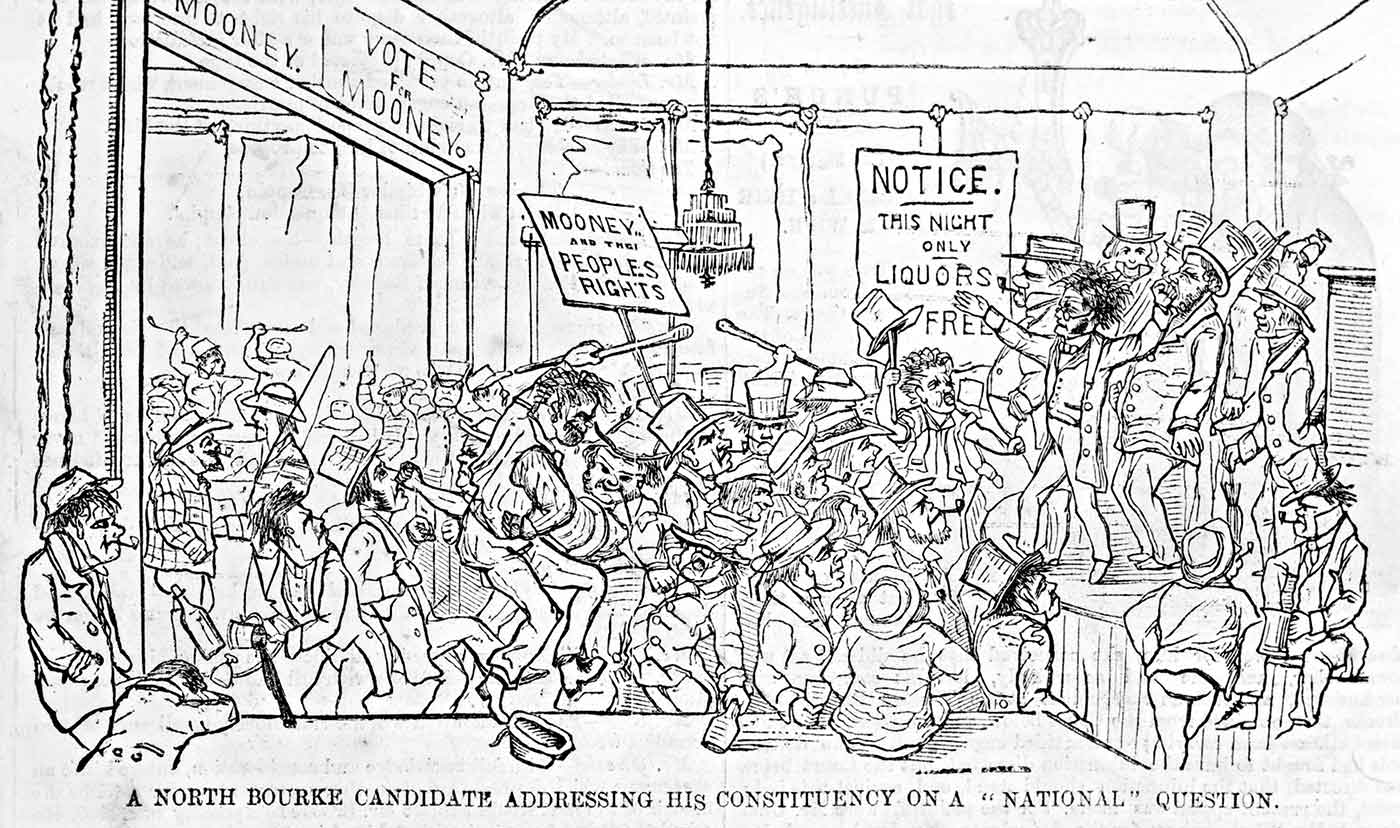
\includegraphics[scale=0.25]{NorthBourke.jpg}
	\caption{Election held in 1855 in Victoria, Australia 
	  was conducted in pub!}
	\end{center}
  \end{figure}   
  
